\section{Quantum Chromodynamics (QCD)}
\begin{figure}
\centering
\begin{tikzpicture}
    \begin{feynman}
      \vertex[dot] (m) at (0, 0) {};
      
      \vertex (a) at (-1.5,-1.5) {$q$};
      \vertex (b) at ( -1.5,1.5) {$\overline{q}$};
      \vertex (c) at (2,0) {$g$};

      \diagram* {
        (a) 
        -- [fermion] (m) 
        -- [fermion] (b),
        (c) 
        -- [gluon] (m),
      };
    \end{feynman}
\end{tikzpicture}
\hspace*{1em}
\begin{tikzpicture}
    \begin{feynman}
      \vertex[dot] (m) at (0, 0) {};
      
      \vertex (a) at (-1.5,-1.5) {$g$};
      \vertex (b) at ( -1.5,1.5) {$g$};
      \vertex (c) at (2,0) {$g$};

      \diagram* {
        (a) 
        -- [gluon] (m) 
        -- [gluon] (b),
        (c) 
        -- [gluon] (m),
      };
    \end{feynman}
\end{tikzpicture}
\hspace*{1em}
\begin{tikzpicture}
    \begin{feynman}
      \vertex[dot] (m) at (0, 0) {};
      
      \vertex (a) at (-1.5,-1.5) {$g$};
      \vertex (b) at ( 1.5,-1.5) {$g$};
      \vertex (c) at (-1.5, 1.5) {$g$};
      \vertex (d) at ( 1.5, 1.5) {$g$};

      \diagram* {
        (a) 
        -- [gluon] (m) 
        -- [gluon] (b),
        (c) 
        -- [gluon] (m) 
        -- [gluon] (d),
      };
    \end{feynman}
  \end{tikzpicture}

\caption{Interaction vertices of quantum chromodynamics: (left) quark-anitquark annihilation to gluon; (middle) three-point gluon vertex; (right) four-point gluon vertex.}
\label{Fig:QCDVertex}
\end{figure}
Quantum chromodynamics (QCD) is the QFT that describes the strong interaction between particles that have color charge which are massive quarks (q) and massless gluons (g). There exist 6 quark flavours:
\begin{itemize}
    \item up u, charm c, and top t (“up-type” quarks)
    \item down d, strange s, and bottom b ("down-type" quarks).
\end{itemize}
where up-type quarks have +2/3 elementary charge and the down-type quarks have -1/3 elementary charge. All quarks carry one specific color charge which comes in three different values: red, green, and blue; their corresponding anti-quark $\overline{\text{q}}$ carries anti-color charge. Gluons form a colour octet which means they carry both a color and an anti-color charge. At its most basic level, the strong interaction is described from quark-gluon couplings and gluon self-couplings as seen in Fig. \ref{Fig:QCDVertex}. At low-energy scales, the interaction strength $\alpha_s$ of these couplings is large $\alpha_s \sim \mathcal{O}(1)$ which results in QCD being a non-perturbative theory at low-energy scales. For this reason (low-energy) QCD processes are not calculable using traditional perturbation theory and require lattice QCD computation techniques. Measurements of the interaction strength $\alpha_s$ show however that the interaction strength depends on the energy scale as seen in Fig.\ref{Fig:interaction strength}. For high energy scales, QCD becomes almost a free theory, a phenomena known as “asymptotic freedom”. At these higher energy scales the interaction strength becomes weak enough that perturbation theory can be successfully applied. This process of decreasing interaction strength $\alpha_s$ with increasing energy scale is called "the running of $\alpha_s$" and is described by a renormalisation group equation (RGE).
\begin{figure}
    \centering
    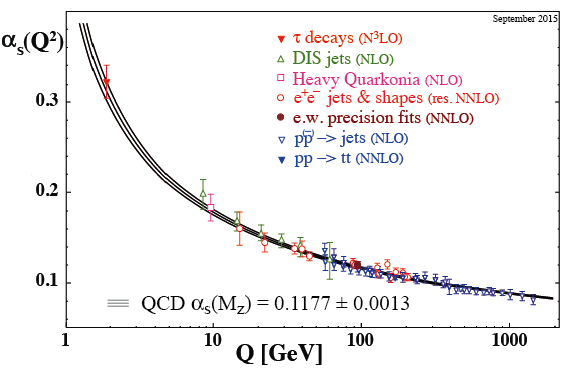
\includegraphics[width=0.5\textwidth]{Figures/Summary-of-measurements-of-a-s-as-a-function-of-the-energy-scale-Q-The-respective-degree.png}
    \caption{Summary of measurements of $\alpha_s$\cite{2015}}
    \label{Fig:interaction strength}
\end{figure}

The parameter $\Lambda_{\text{QCD}}$ is defined as the energy scale, where $\alpha_s$ formally diverges and divides the non-perturbative regime of QCD from the perturbative regime. Because of the strong value of $\alpha_s$ at energies below $\Lambda_{\text{QCD}}$, coloured particles can not exist as free particles, and thus quarks are confined to colour-neutral bound states called hadrons (“color confinement”).\\
\\
Protons (neutrons) are such hadrons that consist of two up-quarks and one down-quark (one up-quark and two down quarks) called the "valance quarks". However the picture of a proton consisting of three valence quarks is overly simplistic.
The quarks inside the proton will interact with each other through the exchange of gluons that in turn give rise to additional quarks and anti-quarks (g$\to$q$\overline{\text{q}}$). These quarks and gluons in the proton are called "sea quarks" and "virtual gluons" and have a net-zero electric charge; this gives the proton an electric charge of +1 from the sum of individual charges of the valence quarks. The complex system of strong interacting "valence quarks" and "sea quarks" (jointly called partons) in the proton make proton-proton (pp) collisions in high-energy particle physics experiments ideal to study the interactions between fundamental particles. High-energy particle physics experiments require predictions for the cross section of proton-proton scattering processes $\sigma(\text{pp}\to\textbf{X})$ which is calculated using a factorisation into soft and hard interactions.

\begin{equation}\label{pp cross section}
    \sigma(\text{pp}\to\textbf{X})(s) = \sum_{\alpha,\beta}\int^1_0{dx_1}\int^1_0{dx_2 f_\alpha(x_1) f_\beta(x_2) \cdot \hat{\sigma}(\alpha \beta \to \text{X})}.
\end{equation}

\begin{figure}
\centering

\begin{tikzpicture}
    \begin{feynman}
      \vertex[dot] (m) at (0, 0) {};
      \vertex[dot] (n) at (2, 0) {};
      \vertex (a) at (-1.5,1) {$q$};
      \vertex (b) at ( -1.5,-1) {$\overline{q}$};
      \vertex (c) at (3.5,1) {$t$};
      \vertex (d) at (3.5,-1) {$\overline{t}$};
        
      \diagram* {
        (a) 
        -- [fermion] (m) 
        -- [fermion] (b),
        (m) 
        -- [gluon] (n)
        -- [fermion] (c),
        (d)
        -- [fermion] (n),
      };
    \end{feynman}
\end{tikzpicture}
\hspace*{1em}
\begin{tikzpicture}
    \begin{feynman}
      \vertex[dot] (m) at (0, 0) {};
      \vertex[dot] (n) at (1, 0) {};
      \vertex (a) at (-2.5,1) {$q$};
      \vertex (b) at ( -2.5,-1) {$\overline{q}$};
      \vertex[dot] (o) at ( -1,0.5) {};
      \vertex[dot] (q) at ( -1,-0.5) {};
      
      \vertex (c) at (2.5,1) {$t$};
      \vertex (d) at (2.5,-1) {$\overline{t}$};
        
      \diagram* {
        (a) 
        -- [fermion] (o) 
        -- [fermion] (q)
        -- [fermion] (b),
        (o)
        -- [gluon] (m)
        -- [gluon] (q),
        (m) 
        -- [gluon] (n)
        -- [fermion] (c),
        (d)
        -- [fermion] (n),
      };
    \end{feynman}
\end{tikzpicture}
\begin{tikzpicture}
    \begin{feynman}
      \vertex[dot] (m) at (0, 0) {};
      \vertex[dot] (n) at (2, 0) {};
      \vertex (a) at (-1.5,1) {$q$};
      \vertex (b) at ( -1.5,-1) {$\overline{q}$};
      \vertex (c) at (3.5,1) {$t$};
      \vertex (d) at (3.5,-1) {$\overline{t}$};
      \vertex (g) at (0.5,0.5) {$g$};
      \vertex (o) at (-0.75, 0.5) {};
      \diagram* {
        (a) 
        -- [fermion] (m) 
        -- [fermion] (b),
        (m) 
        -- [gluon] (n)
        -- [fermion] (c),
        (d)
        -- [fermion] (n),
        (o)
        -- [gluon] (g),
      };
        
    \end{feynman}
\end{tikzpicture}
\caption{Examples of Feynman diagrams for top quark pair production at leading order (left) and next-to-leading order with loop correction (right) and gluon emission (center)}
\label{Fig:LONLO}
\end{figure}
The hard interaction refers to high-energy parton-parton interactions between the protons with high transverse energy and is described by the partonic cross section $\hat{\sigma}(\alpha \beta \to \text{X})$ in \ref{pp cross section}. At high-energy this cross section can be calculated with perturbative QCD. Leading order (LO) calculation in QCD involves the lowest order QCD interaction strength $\alpha_s$. These LO calculations involve only tree-level Feynman diagrams. Next-to-leading order (NLO) calculations involve the inclusion of the next order term in $\alpha_s$. NLO calculations are more complex due to virtual particle exchanges and loop diagrams in addition to tree-level diagrams. Examples of both LO and NLO Feynman diagrams for top quark pair production are shown in Fig. \ref{Fig:LONLO}. 
The soft interaction then refers to the exchange of low-energy particles and is described by the parton distribution functions $f_\alpha(x)$ (PDFs) of the proton, which provide a probability distribution for finding a parton $\alpha$ with momentum fraction $x$ in the proton. These PDFs are dependent on momentum fraction $x$ and on the momentum transfer $Q$ in the process. PDFs are required to predict proton-proton scattering rates however unlike the partonic cross section $\hat{\sigma}(\alpha \beta \to \text{X})$ PDFs must be obtained from measurements in deep-inelastic scattering (DIS) experiments. They are extracted from a global fit to experimental data obtained in Electron-proton DIS at the Hadron-Electron Ring Accelerator (HERA), proton-antiproton DIS at Tevatron, and proton-proton DIS at LHC. Proton PDFs at $Q^2=10$GeV$^2$ can be seen in Fig. \ref{fig:PDFs}. One can see that gluon distribution dominates the PDFs and increases rapidly at lower momentum $x$. Therefore in high energy pp collisions at LHC the scattering processes are dominated by gluon-gluon interactions. High energy quarks and gluons produced in these proton-proton collisions can in turn create additional quarks and gluons trough the strong interaction; this phenomena is known as a gluon shower or parton shower. As the parton shower continues, the energy of the particles decreases, and eventually they will have insufficient energy to create new particles through the strong interaction. At this point, the particles will undergo a process known as hadronization, where the quarks and gluons combine to form color-neutral hadrons, such as protons, neutrons, pions, and other mesons. The bundle of these hadrons collimated in the direction of the original high-energy quark or gluon before parton shower is called a "jet" and plays an important role in high energy physics experiments.
\begin{figure}
    \centering
    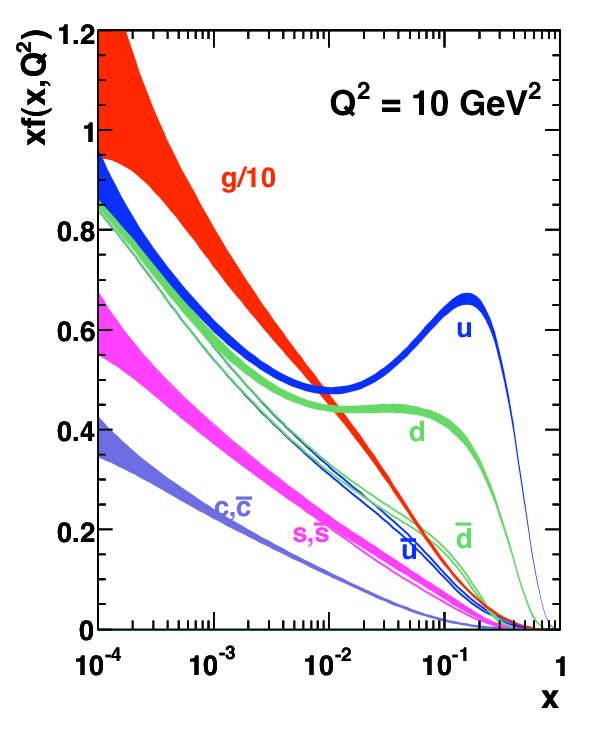
\includegraphics[width=0.5\textwidth]{Figures/The-parton-distribution-function-PDF-describes-the-probability-density-of-finding.png}
    \caption{Parton Distribution Functions at $Q^2=10$GeV$^2$\cite{Martin_2009}}
    \label{fig:PDFs}
\end{figure}